\section{Design}
\label{sec:design}

\subsection{Program structure}
\label{ssec:struct}

\subsubsection{Databases}
\label{sssec:db}

There are three tables in the project, which are the following ones:

\begin{itemize}[noitemsep]
\item drinks: contains all the predefined drinks that the user can select;
\item drink\_records: contains the drinks selected by the current user;
\item users: contains all informations about the different users.
\end{itemize}

We also needed queries to fill the \guillemotleft{} drinks \guillemotright{} database, they are all written in a SQL script called list\_drinks.sql.

\subsubsection{Java}
\label{sssec:java}

The project consists in three main classes, Drink.java, DrinkRecord.java and User.java. Their respective UML representations are given by {\sc figures} \ref{fig:drinkJava}, \ref{fig:drinkRecordJava} and \ref{fig:userJava}.\\

The calculation methods, calculateBAC() and hoursUntilSober(double), are implemented in User.java. They are based on the formulas previously introduced in {\sc section}~\ref{sec:spec}. 

\begin{figure}[H]
\centering
   \includegraphics{./figures/drink.png}
   \caption{Class Drink.java, its attributes and its methods}
   \label{fig:drinkJava}
\end{figure}

\begin{figure}[H]
\centering
   \includegraphics{./figures/drinkRecord.png}
   \caption{Class DrinkRecord.java, its attributes and its methods}
   \label{fig:drinkRecordJava}
\end{figure}

\begin{figure}[H]
\centering
   \includegraphics{./figures/user.png}
   \caption{Class User.java, its attributes and its methods}
   \label{fig:userJava}
\end{figure}

\subsubsection{Web content}
\label{sssec:server}

The web content is located in the file Index.xhtml. It is used to generate different URLs based on the session ID. This means that instead of creating a new page for each user, it is just redirected to the page with the right session ID.\\

The web content also includes a folder called WEB-INF, that contains two files: web.xml and faces-config.xml. They are used to manage the server and to handle the Java beans.

\subsection{User interface}
\label{ssec:ui}

Three main elements were needed in Beerculator's interface : one to get the user information (weight, gender, etc), one to display the list of drinks and one to show the results. The user interface can be seen on {\sc figure}~\ref{fig:ui}.\\

\begin{figure}[H]
\centering
   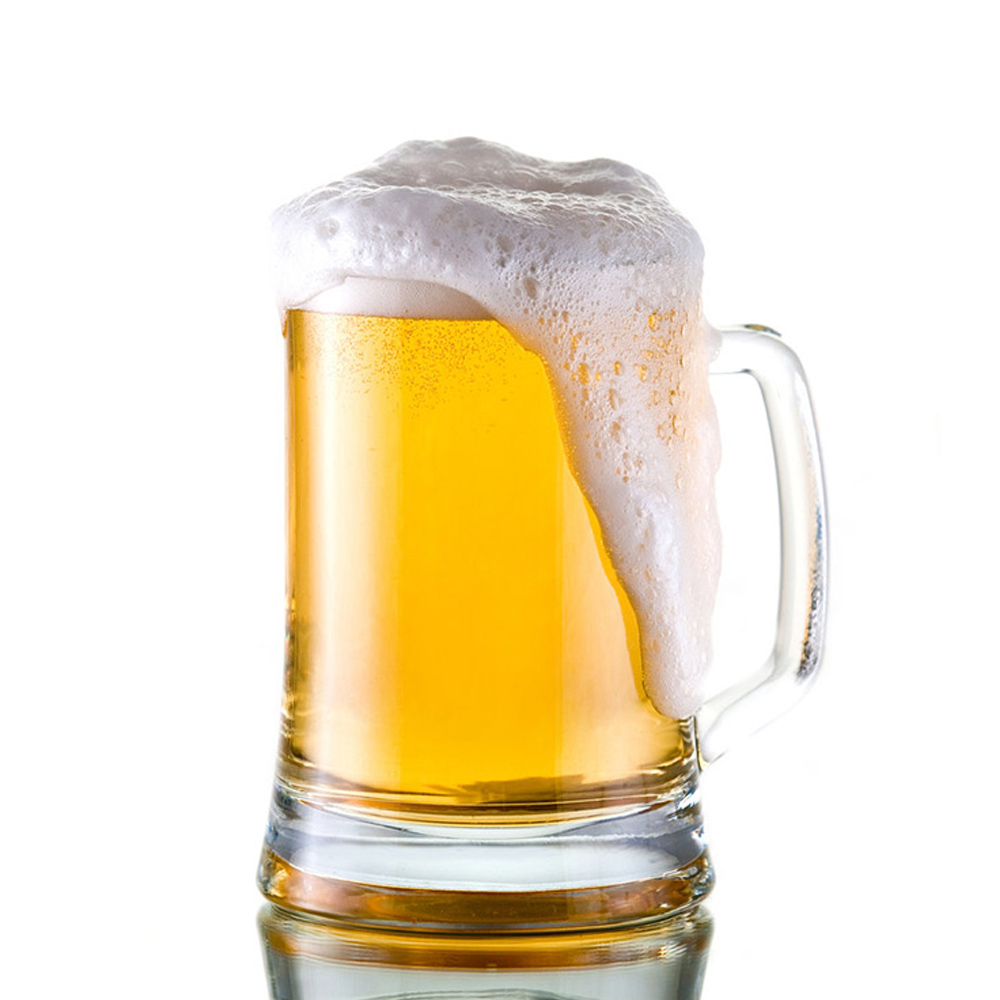
\includegraphics[scale=0.3]{./figures/beer.jpg}
   \caption{User interface of Beerculator}
   \label{fig:ui}
\end{figure}

On the top left part of the interface, the user can add all informations that Beerculator needs from him. He can indicate its gender (male or female) via two check boxes, and its weight thanks to a text box. Another text box is available for him to tell the time that he started drinking. He can also save all those informations, in case he has to close the page and wants to come back later.\\

On the right side of the web page, the user can see a list of predefined drinks (with their volume and their alcohol percentage). With each alcohol there are two squares: one green and on red. The user can click on the green one to add one item of the corresponding alcohol to his list of drinks. If he clicks on the red button, one item of this alcohol is removed from the list of drinks. He can also save his list of drinks, for instance if the party is not over and he intends to add some more later in the night.\\

When he is done, the user can click on the \guillemotleft{} Calculate \guillemotright{} button so that Beerculator starts the computation. The results appear on the bottom left corner, in the \guillemotleft{} Calculation \guillemotright{} tab. First the BAC value is indicated, and below it the number of hours before the user gets sober again.
